% The binary search of place() in a node of eleven keys for x = 27 (sec.
% 23.3; the data of the figure findIt(a, 27) of Morin's book): the four
% probes of std::lower_bound, in order, and the first place of a key >= 27. Build: make figures (in
% ../build).
\documentclass[border=4pt]{standalone}
\usepackage[T1]{fontenc}
\usepackage{lmodern}
\usepackage{amsmath,amssymb}
\usepackage{tikz}
\usepackage{lamalunga}
% tikz-ads.tex: the TikZ styles shared by the figures of the memory of the
% manual, \input by each standalone figure: a cell of a vector (cell), the
% cell that an operation touches (touched), a free cell (free), a node of a
% linked structure (node), the labels of indices (index) and of variables
% (var), a pointer (ptr), and \cells and \indices to draw a row of cells.
\usetikzlibrary{arrows.meta,positioning,calc,fit,shapes.multipart}
\definecolor{adsTouched}{RGB}{214,196,236}
\definecolor{adsFree}{RGB}{236,236,236}
\tikzset{
  ads/.style={>={Stealth[length=2mm]},font=\small,
              every node/.append style={inner sep=0pt}},
  cell/.style={draw,minimum width=7mm,minimum height=7mm,
               font=\small\ttfamily,outer sep=0pt},
  touched/.style={cell,fill=adsTouched},
  free/.style={cell,fill=adsFree,text=black!45},
  node/.style={draw,rounded corners=1pt,minimum width=8mm,
               minimum height=6mm,font=\small\ttfamily},
  index/.style={font=\scriptsize\ttfamily,text=black!60},
  var/.style={font=\small\itshape},
  ptr/.style={->,thick}
}
% \cells{name}{x,y}{list}: a row of cells, the first at (x,y), named
% name-0, name-1, ...; each item is text/style, the style one of cell,
% touched and free (e.g., {a/cell,e/touched,/free})
\newcommand{\cells}[3]{%
  \foreach \v/\s [count=\i from 0] in {#3}
    \node[\s] (#1-\i) at ($(#2)+(\i*7mm,0)$) {\v};}
% \indices{name}{n}: the indices 0 .. n-1 under the cells of name
\newcommand{\indices}[2]{%
  \foreach \i in {0,...,\numexpr#2-1\relax}
    \node[index,below=1.2mm of #1-\i] {\i};}

\begin{document}
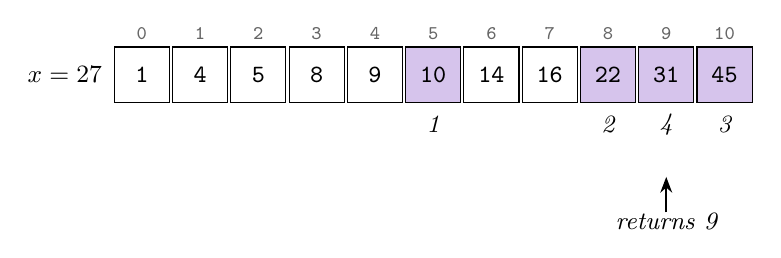
\begin{tikzpicture}[ads]
  \node[cell] (k-0) at (0mm,0) {1};
  \node[index] at (0mm,5.2mm) {0};
  \node[cell] (k-1) at (7.4mm,0) {4};
  \node[index] at (7.4mm,5.2mm) {1};
  \node[cell] (k-2) at (14.8mm,0) {5};
  \node[index] at (14.8mm,5.2mm) {2};
  \node[cell] (k-3) at (22.2mm,0) {8};
  \node[index] at (22.2mm,5.2mm) {3};
  \node[cell] (k-4) at (29.6mm,0) {9};
  \node[index] at (29.6mm,5.2mm) {4};
  \node[touched] (k-5) at (37mm,0) {10};
  \node[index] at (37mm,5.2mm) {5};
  \node[var] at (37mm,-6.4mm) {1};
  \node[cell] (k-6) at (44.4mm,0) {14};
  \node[index] at (44.4mm,5.2mm) {6};
  \node[cell] (k-7) at (51.8mm,0) {16};
  \node[index] at (51.8mm,5.2mm) {7};
  \node[touched] (k-8) at (59.2mm,0) {22};
  \node[index] at (59.2mm,5.2mm) {8};
  \node[var] at (59.2mm,-6.4mm) {2};
  \node[touched] (k-9) at (66.6mm,0) {31};
  \node[index] at (66.6mm,5.2mm) {9};
  \node[var] at (66.6mm,-6.4mm) {4};
  \node[touched] (k-10) at (74mm,0) {45};
  \node[var] at (74mm,-6.4mm) {3};
  \node[index] at (74mm,5.2mm) {10};
  \node[var,anchor=east] at (-5mm,0) {$x = 27$};
  \draw[ptr] (k-9.south) ++(0,-14mm) node[var,below] {returns 9} -- ++(0,4.5mm);
\end{tikzpicture}
\end{document}
